% This must be in the first 5 lines to tell arXiv to use pdfLaTeX, which is strongly recommended.
\pdfoutput=1
% In particular, the hyperref package requires pdfLaTeX in order to break URLs across lines.

\documentclass[11pt]{article}

% Remove the "review" option to generate the final version.
% \usepackage[review]{ACL2023}
\usepackage[]{ACL2023}
\usepackage{float}
\usepackage{placeins}
\usepackage{graphicx}
\usepackage{pgfplots}
\pgfplotsset{compat=1.18}
\usepackage{tikz}
\usepackage{amsmath}    
% Standard package includes

\usepackage{times}
\usepackage{latexsym}
\usepackage{booktabs}
\usepackage{array}
\usepackage{tabularx}
\usepackage{placeins}
\usepackage{hyperref}
% For proper rendering and hyphenation of words containing Latin characters (including in bib files)
\usepackage[T1]{fontenc}
% For Vietnamese characters
% \usepackage[T5]{fontenc}
% See https://www.latex-project.org/help/documentation/encguide.pdf for other character sets

% This assumes your files are encoded as UTF8
\usepackage[utf8]{inputenc}
% \usepackage[a4paper, margin=1in]{geometry} 
% This is not strictly necessary, and may be commented out.
% However, it will improve the layout of the manuscript,
% and will typically save some space.
\usepackage{microtype}

% This is also not strictly necessary, and may be commented out.
% However, it will improve the aesthetics of text in
% the typewriter font.
\usepackage{inconsolata}

\usepackage{listings}

% If the title and author information does not fit in the area allocated, uncomment the following
%
%\setlength\titlebox{<dim>}
%
% and set <dim> to something 5cm or larger.

\title{Minding the LLM Gap: MultiBERT's Performances on Text from Different Languages Replication}


% \usepackage[a4paper, margin=1in]{geometry} % Adjust margins for smaller size


\usepackage[svgnames]{xcolor}   
\newcommand{\advice}[1]{\textcolor{MediumPurple}{[#1]}}


\author{
  \begin{minipage}[t]{0.45\textwidth}
    \centering
    Jaanhvi Agarwal \\
    Colgate University \\
    \texttt{jagarwal@colgate.edu}
  \end{minipage}
  \hfill
  \begin{minipage}[t]{0.45\textwidth}
    \centering
    Sarah Cryan \\
    Colgate University \\
    \texttt{scryan@colgate.edu}
  \end{minipage}
}


\begin{document}
\maketitle

\begin{abstract}
% The abstract should be very short (Approximately 5 sentences. No more than 10 sentences). It should describe briefly the main question, the method used, the main takeaway results and implications of these results. 





This paper replicates a multilingual syntactic evaluation using monolingual and multilingual BERT models, applying them to the Cross-Linguistic Assessment of Models on Syntax (CLAMS) five-language dataset \cite{clams}. Our evaluation focuses on both simple and complex syntactic structures. The results show that monolingual BERT consistently outperforms multilingual BERT, particularly on more complex syntactic tasks, such as relative clauses and prepositional phrases. Yet, both models perform similarly on simpler tasks. Notably, our replication successfully generated results the original study could not produce, indicating that improvements in dataset preparation enhanced model evaluations. These findings encourage further research on that addressing language-specific syntactic nuances to help improve multilingual model performance, especially for non-Latin scripts \cite{Arivazhagan2019MassivelyMN} and more complex syntactic dependencies. Future work could explore fine-tuning architectures or adapting models for diverse script systems \cite{clark2022canine} to enhance cross-linguistic generalization.
\end{abstract}

\begin{figure*}[t]
    \centering
    \includegraphics[width=\textwidth]{pipeline_diagram.png}
    \caption{Pipeline for the NLP Scholar Experiment}
    \label{fig:pipeline}
\end{figure*}

\section{Introduction}
Current language modeling demonstrates greater success with monolingual word prediction than in the past, particularly seen in a model’s ability to identify sentence structures. However, the training datasets used for these models may not present sufficient complexity to further enhance performance. To address this gap, this paper, along with the study it replicates, incorporates additional languages—specifically French, Hebrew, German, and Russian—to provide more challenging syntactic structures.  Although these languages differ in vocabulary and script, they share some syntactic rules, offering more diverse examples of complex sentence structures. This diversity allows models to learn new linguistic patterns and improves their ability to generalize across languages. 

The original study developed the Cross-Linguistic Assessment of Models on Syntax (CLAMS) dataset \cite{clams}, which expanded on \cite{Marvin2018TargetedSE}'s dataset of minimally different English sentences (ungrammatical vs. grammatical). By introducing minimally different French, German, Hebrew, and Russian sentences, CLAMS provides a more comprehensive multilingual dataset. This allows for a deeper evaluation of language models’ abilities to handle complex grammatical constructions across different languages. Examples of increasingly complex sentence structures can be seen below:

\begin{table}[h!]
\centering
\small % Makes the table even smaller
\setlength{\tabcolsep}{3pt} % Reduce horizontal padding between columns
\renewcommand{\arraystretch}{1.1} % Reduce space between rows
\begin{tabular}{p{3.5cm}p{5.5cm}} % Adjust column widths for better fit
\toprule
\textbf{Structure Type} & \textbf{Example} \\ 
\midrule
Simple Agreement & The cat chases the mouse. \\ 
VP Coordination (Short) & The cat chased the mouse and caught it. \\ 
VP Coordination (Long) & The cat chased the mouse, climbed the tree, and jumped across the fence. \\ 
Across Subject Relative Clause & The cat that chased the mouse is sitting on the couch. \\ 
Within Object Relative Clause & The cat chased the mouse that was hiding in the hole. \\ 
Across Object Relative Clause & The cat that the dog chased is now hiding under the couch. \\ 
Across Prepositional Phrase & The cat on the mat near the window chased the mouse. \\ 
\bottomrule
\end{tabular}
\label{tab:Table1}
\caption{Types of Sentence Structures with Examples}
\end{table}


The original research evaluated both LSTM and transformer architectures, including monolingual BERT and multilingual BERT (mBERT). The results showed that LSTM models accurately distinguished correct from incorrect subject-verb agreement but struggled with more complex structures, such as center-embedded clauses. Surprisingly, training LSTM models on multiple languages introduced language interference, reducing overall performance. The researchers suggested that different architectures might better handle this issue.

In contrast, transformer models like BERT showed a higher level of generalization, with monolingual BERT outperforming mBERT on complex syntactic structures. mBERT did perform well on certain grammatical tasks, but monolingual BERT was consistently more sensitive to syntactic nuances, particularly in languages with more grammatical complexity.

In this replication study, we recreated the multilingual CLAMS dataset and focused on evaluating monolingual BERT and mBERT models. While the original study also included LSTM models, we chose to concentrate on BERT due to our prior experience with transformer models. By making some necessary formatting adjustments to the dataset, we successfully replicated the evaluation process and observed similar trends. Our results confirmed that monolingual BERT consistently achieved higher accuracy, particularly with complex syntactic structures, than mBERT, and both models performed comparably well on simpler grammatical tasks. While there was some differences between the accuracy scores of the original paper and our replication paper, there were similar trends in which grammar, languages, and models had higher or lower accuracy scores.

To illustrate the steps of our replication experiment, \autoref{fig:pipeline} provides an overview of the pipeline we followed. This pipeline outlines the stages from dataset preparation, model selection, and evaluation, through to the final analysis of accuracy scores across different grammatical categories and languages. While these methods produced minor differences in accuracy between our replication and the original study, the general trends and findings remained consistent and can be seen in \autoref{tab:Table2} and \autoref{tab:Table3}.

\section{Background}
The original paper and our replication paper rely on understanding what a well-performing model means and how we are able to analyze a grammatical rule across multiple languages.

A well-performing language model accurately distinguishes between grammatical and ungrammatical sentences, often tested with example pairs such as "the cat eats" (correct) versus "the cat eat" (incorrect). The model predicts the next word based on prior context, so a well-performing model would recognize that "eat" is an incorrect prediction after "cat," demonstrating an understanding of subject-verb-agreement. A singular subject, like "cat," must be followed by a singular verb form, such as "eats." Evaluating whether the model made the correct choice mirrors human native-speaker judgments, where a good model can intuitively differentiate between correct and incorrect language constructions, much like a native speaker would.

In the original study, two types of language models were used: LSTM (a type of sequential neural network) and BERT (a transformer-based model). LSTMs store and recall information across sequences of words, relying on previous context to predict the next word. In contrast, BERT uses a bidirectional approach, where it analyzes the entire sentence context to predict words. This allows BERT to capture more complex relationships between words and handle syntactic dependencies better than LSTMs in certain scenarios.

Evaluating a model's ability to generalize across multiple languages adds complexity to the analysis. Each language has unique syntactic structures and rules that models must learn. To test how well these models handle cross-linguistic syntactic variation, the original study used Attribute-Varying Grammars (AVGs). AVGs generate sentence pairs—one grammatical, one ungrammatical—by modifying specific features such as verb conjugations or word order. For example, in French, the AVG framework might produce "je pense" (correct) and "je penses" (incorrect) to test the model's understanding of verb agreement. This method allows for consistent syntactic evaluation across multiple languages, enabling researchers to assess how well a model can generalize grammar rules beyond a single language.

While multilingual models like mBERT can generalize across different languages, they often struggle with language-specific syntactic rules due to potential language interference. For instance, a model trained on multiple languages may learn general patterns that do not fully capture the intricacies of any single language's syntax. In contrast, monolingual models, such as BERT trained on English, tend to perform better on complex syntactic tasks within their target language. Understanding how these models handle grammatical variations across languages is crucial for improving their robustness and applicability in multilingual NLP tasks.

\section{Methods}
Our replication study evaluated language models with the same goal as the original study, to determine their ability to distinguish grammatical from ungrammatical sentences using new, larger, challenging datasets. We compared monolingual and multilingual model performance across different languages and syntactic constructions, using datasets generated from attribute-varying grammars (AVGs).

\subsection{Models}
We used BERT for our models, testing monolingual BERT for evaluating English and using multilingual BERT for evaluating all 5 languages (English, French, German, Hebrew, and Russian). Using these models allowed us to test and observe how well multiple languages improve the models' performance and allowed us to work with a familiar model architecture.

\subsection{Datasets}
We relied on the same CLAMS dataset generated in the original study, but we modified the data to fit our specific format for running NLPScholar, a toolkit for running natural language processing experiments \cite{prasad-davis-2024-training-nlp}. We created a script that changed the original format [true/false] [sentence] to follow the NLPScholar format: [sent id] [condition] [context id] [pair id] [comparison] [lemma] [sentence] [Region Of Interest]. These necessary changes allowed us to run evaluate and analyze on the sentences from CLAMS. Our datasets can be found \href{https://drive.google.com/drive/folders/1qSvXkoO3KI0APpjeOCd6oRJzvyi1ytJo?usp=sharing}{here}.

This modification was necessary to ensure compatibility with the MinimalPair analysis, which performs binary comparisons (e.g., grammatical vs. ungrammatical) by measuring the predictability or surprisal of words in sentences. The toolkit requires two types of TSV files:
\begin{enumerate}
    \item \textbf{Predictability TSV}: Contains sub-word token information, probabilities, and surprisal values.
    \item \textbf{Data TSV}: Contains sentence-level information, including IDs for sentences, pairs, and contexts, along with the comparison (expected/unexpected).
\end{enumerate}

These files are generated by running the NLPScholar toolkit using a configuration file that specifies the dataset paths, models to be used, and evaluation measures. The configuration file, written in YAML format, defines the details of the experiment, including the type of model used (e.g., multilingual BERT), the location of the input datasets, and the method for computing predictability (e.g., surprisal). A sample configuration is shown below:
\lstset{
    basicstyle=\ttfamily\small, % Use small monospaced font for code
    keywordstyle=\color{blue}\bfseries, % Keywords in bold blue
    commentstyle=\color{gray}\itshape, % Comments in italic gray
    breaklines=true, % Automatic line breaking for long lines
    frame=single, % Adds a frame around the code
    morekeywords={exp, mode, models, datafpath, predfpath, resultsfpath, pred_measure, batchSize} % Define your custom keywords
}
\begin{lstlisting}[caption={NLPScholar Configuration Example}, label={lst:config}]
exp: MinimalPair

mode: 
    - evaluate
    - analyze
    
models:
  hf_masked_model:
    - google-bert/bert-base-multilingual-cased
    - google-bert/bert-base-uncased      
    
datafpath: /path/to/eval_dataset.tsv
predfpath: /path/to/predictions.tsv
resultsfpath: /path/to/summary.tsv

pred_measure: surp
\end{lstlisting}

% This configuration file provides a flexible way to run multiple experiments by specifying different models, datasets, and evaluation methods. In our case, it generates the TSV files used for further analysis by computing surprisal scores and other linguistic metrics.

These changes allowed us to run more detailed evaluations, where the predictability of specific words could be compared across different syntactic structures. By restructuring the data, we were able to replicate the experiments from the original paper, but with the enhanced flexibility and functionality provided by the \textit{NLPScholar} toolkit. The scripts and config files used to transform the dataset can be found in our GitHub repository at \url{https://github.com/Jaanhvi18/clams---Midterm-Replication-NLP.git}.



% *****Ideally you will also include a github link to the code that generates the dataset. As with the model, if you are making choices the diverge from the original paper, justify the choices \advice{If your paper involves training and evaluating models, then describe both of these datasets separately and consider having the be different subsections.}

\begin{table*}[htbp]
\centering
\caption{Results from the replication using NLPScholar: Multilingual BERT accuracies across different languages and constructions.}
\begin{tabularx}{\textwidth}{@{}lXXXXXX@{}}
\toprule
                        & \textbf{English} & \textbf{French} & \textbf{German} & \textbf{Hebrew} & \textbf{Russian} \\ \midrule
\textbf{Simple agreement}                & \textbf{0.78}    & \textbf{0.76}   & \textbf{0.84}   & \textbf{0.72}    & 0.78            \\
\textbf{VP coordination (short)}         & \textbf{0.82}    & \textbf{0.78}   & 0.90            & 0.76           & 0.79            \\
\textbf{VP coordination (long)}          & 0.81             & 0.86            & \textbf{0.93}   & 0.83             & 0.90             \\
\textbf{Across subject relative clause}  & 0.55             & 0.56            & 0.61            & 0.64            & 0.75            \\
\textbf{Within object relative clause}   & 0.58             & 0.75            & 0.50            & 0.52           & 0.67             \\
\textbf{Across object relative clause}   & 0.56             & 0.57            & \textbf{0.57}   & 0.53           & 0.76            \\
\textbf{Across prepositional phrase}     & 0.57             & 0.53            & \textbf{0.75}   & 0.55           & 0.68            \\ \bottomrule
\end{tabularx}
\label{tab:Table2}
\end{table*}

% (**?**)Describe what approach you used to analyze the output from the model. Make sure to explain why this analysis method is appropriate to answer the question this paper is studying. 

\subsection{Evaluation}

For the evaluation of our models, we utilized the \textit{NLPScholar} toolkit, which allowed us to compare the predictability and surprisal of words across different syntactic structures and languages. The evaluation followed a binary comparison method between grammatical and ungrammatical sentence pairs, derived from the \textit{Cross-Linguistic Assessment of Models on Syntax (CLAMS) dataset}.

Our analysis focused on comparing the performances of \textit{monolingual BERT} (trained on English) and \textit{multilingual BERT} (trained on multiple languages) across a diverse set of syntactic constructions such as subject-verb agreement, VP coordination, and relative clauses. We structured the evaluation based on the following steps:

    \begin{itemize}
    \item \textbf{Predictability TSV and Data TSV Generation}: Using the NLPScholar toolkit, we generated these two types of TSV files:

    \item \textbf{Evaluation Metrics}: The primary metric used to assess model performance was \textit{accuracy}, which measured how effectively the models distinguished between grammatical and ungrammatical sentences. Additionally, we assessed \textit{surprisal values} to quantify how unexpected a word is in its syntactic context based on the model's training data. A lower surprisal score indicates a more predictable word within the given context, suggesting better syntactic understanding by the model. We used surprisal differences between grammatical and ungrammatical sentence pairs to determine the model’s ability to capture syntactic nuances. 

    \item \textbf{Syntactic Complexity Focus}: Our evaluation focused on both simpler constructions, such as \textit{subject-verb agreement} and \textit{VP coordination}, and more complex structures like \textit{relative clauses} and \textit{prepositional phrases}. This range enabled us to assess how the models handle basic grammar rules as well as more intricate syntactic dependencies.
    
    \item \textbf{Cross-Linguistic Comparison}: We evaluated multilingual BERT on five languages: English, French, German, Hebrew, and Russian. By comparing the model's performance across these structurally diverse languages, we aimed to assess how well it generalized syntactic rules across languages, each with varying degrees of similarity to English.

    % \item \textbf{Key Findings}:
    % \begin{itemize}
    %     \item \textit{Monolingual BERT} consistently outperformed \textit{multilingual BERT} on complex syntactic structures like \textit{relative clauses} and \textit{prepositional phrases}. For simpler constructions, such as \textit{VP coordination}, both models achieved high accuracy, though monolingual BERT held a slight advantage.
    %     \item \textit{Multilingual BERT} struggled with language-specific syntactic rules, particularly in \textit{Hebrew} and \textit{Russian}, where grammatical structures differ significantly from English. For example, in \textit{across-subject relative clauses}, monolingual BERT achieved higher accuracy (0.76) compared to multilingual BERT (0.62).
    %     \item Unlike the original study, our replication successfully computed results for constructions previously marked as out-of-vocabulary. This suggests that improvements in dataset preprocessing and word coverage may have contributed to more comprehensive evaluation results.
    % \end{itemize}
\end{itemize}

This combination of steps allowed us to best evaluate the performance of our models across multiple languages and sentence structures.

\begin{table}[h!]
\centering

\begin{tabular}{lll}
\hline
\textbf{ } & \textbf{Mono} & \textbf{Multi} \\ 
\hline
\textbf{Subject-Verb Agreement} & & \\
Simple & 0.79 & 0.78 \\
VP coordination (short) & 0.89 & 0.81 \\
VP coordination (long) & \textbf{0.98} & 0.87 \\
Across subject rel. clause & 0.76 & \textbf{0.62} \\
Within object rel. clause & \textbf{0.83} & 0.60 \\
Across object rel. clause & \textbf{0.74} & 0.60 \\
Across prepositional phrase & 0.72 & \textbf{0.62} \\
\hline
\textbf{Average accuracy} & \textbf{0.82} & \textbf{0.70} \\ 
\end{tabular}
\caption{\label{citation-guide}
Results from the replication using NLPScholar: Monolingual BERT accuracies compared to Multilingual BERT accuracies averaged across all 5 languages.
}
\label{tab:Table3}
\end{table}
\section{Results}
Our replication study yielded results that are largely in line with the findings from the original study, with some notable differences. We evaluated the performance of both monolingual BERT (trained on English) and multilingual BERT (trained on multiple languages), focusing on their ability to distinguish between grammatical and ungrammatical sentences across different languages and syntactic structures. Below, we present our findings in comparison to the original study's results.


\begin{figure}[htbp]
    \centering
    \includegraphics[width=0.45\textwidth]{SA_VP_comparison.png}
    \caption{Comparison of Simple Agreement and VP Coordination (Short) - Original vs Replication Across Languages}
    \label{fig:simple-agreement}
\end{figure}

\paragraph{Simple Agreement and VP Coordination}

In our replication, all five languages achieved high accuracy (> 0.70) in simpler syntactic constructions such as \textit{simple agreement}, \textit{VP coordination (short)}, and \textit{VP coordination (long)}, as shown in \autoref{tab:Table2}. While slightly lower than the original paper’s results, our findings using \textit{NLPScholar} remain strong. For \textit{VP coordination (long)}, the accuracies were 0.81 for English, 0.86 for French, 0.93 for German, 0.83 for Hebrew, and 0.90 for Russian, all within 0.12 of the original study's results, demonstrating similar performance between our results and the original paper, as seen in \autoref{fig:simple-agreement}. The results also indicate multilingual BERT's relatively strong ability to handle these structures across diverse languages.

\paragraph{Across subject relative clause and Across prepositional phrase}
There were also lower accuracies in certain complex syntactic constructions, similar to the original paper’s results, such as \textit{across subject relative clauses} and \textit{across prepositional phrases} \autoref{tab:Table2}. For \textit{across subject relative clauses}, the replication accuracies were 0.55 for English, 0.56 for French, 0.61 for German, 0.64 for Hebrew, and 0.75 for Russian. These results align with the lower accuracies reported in the original paper as can be seen in \autoref{fig:sr_pp_comparison}, further highlighting the challenges faced by the models in handling more complex structures. Similarly, for across prepositional phrases, the replication accuracies were 0.57 for English, 0.53 for French, 0.75 for German, 0.55 for Hebrew, and 0.68 for Russian, demonstrating a mix of lower and higher scores across the two papers.


\begin{figure}[htbp]
    \centering
    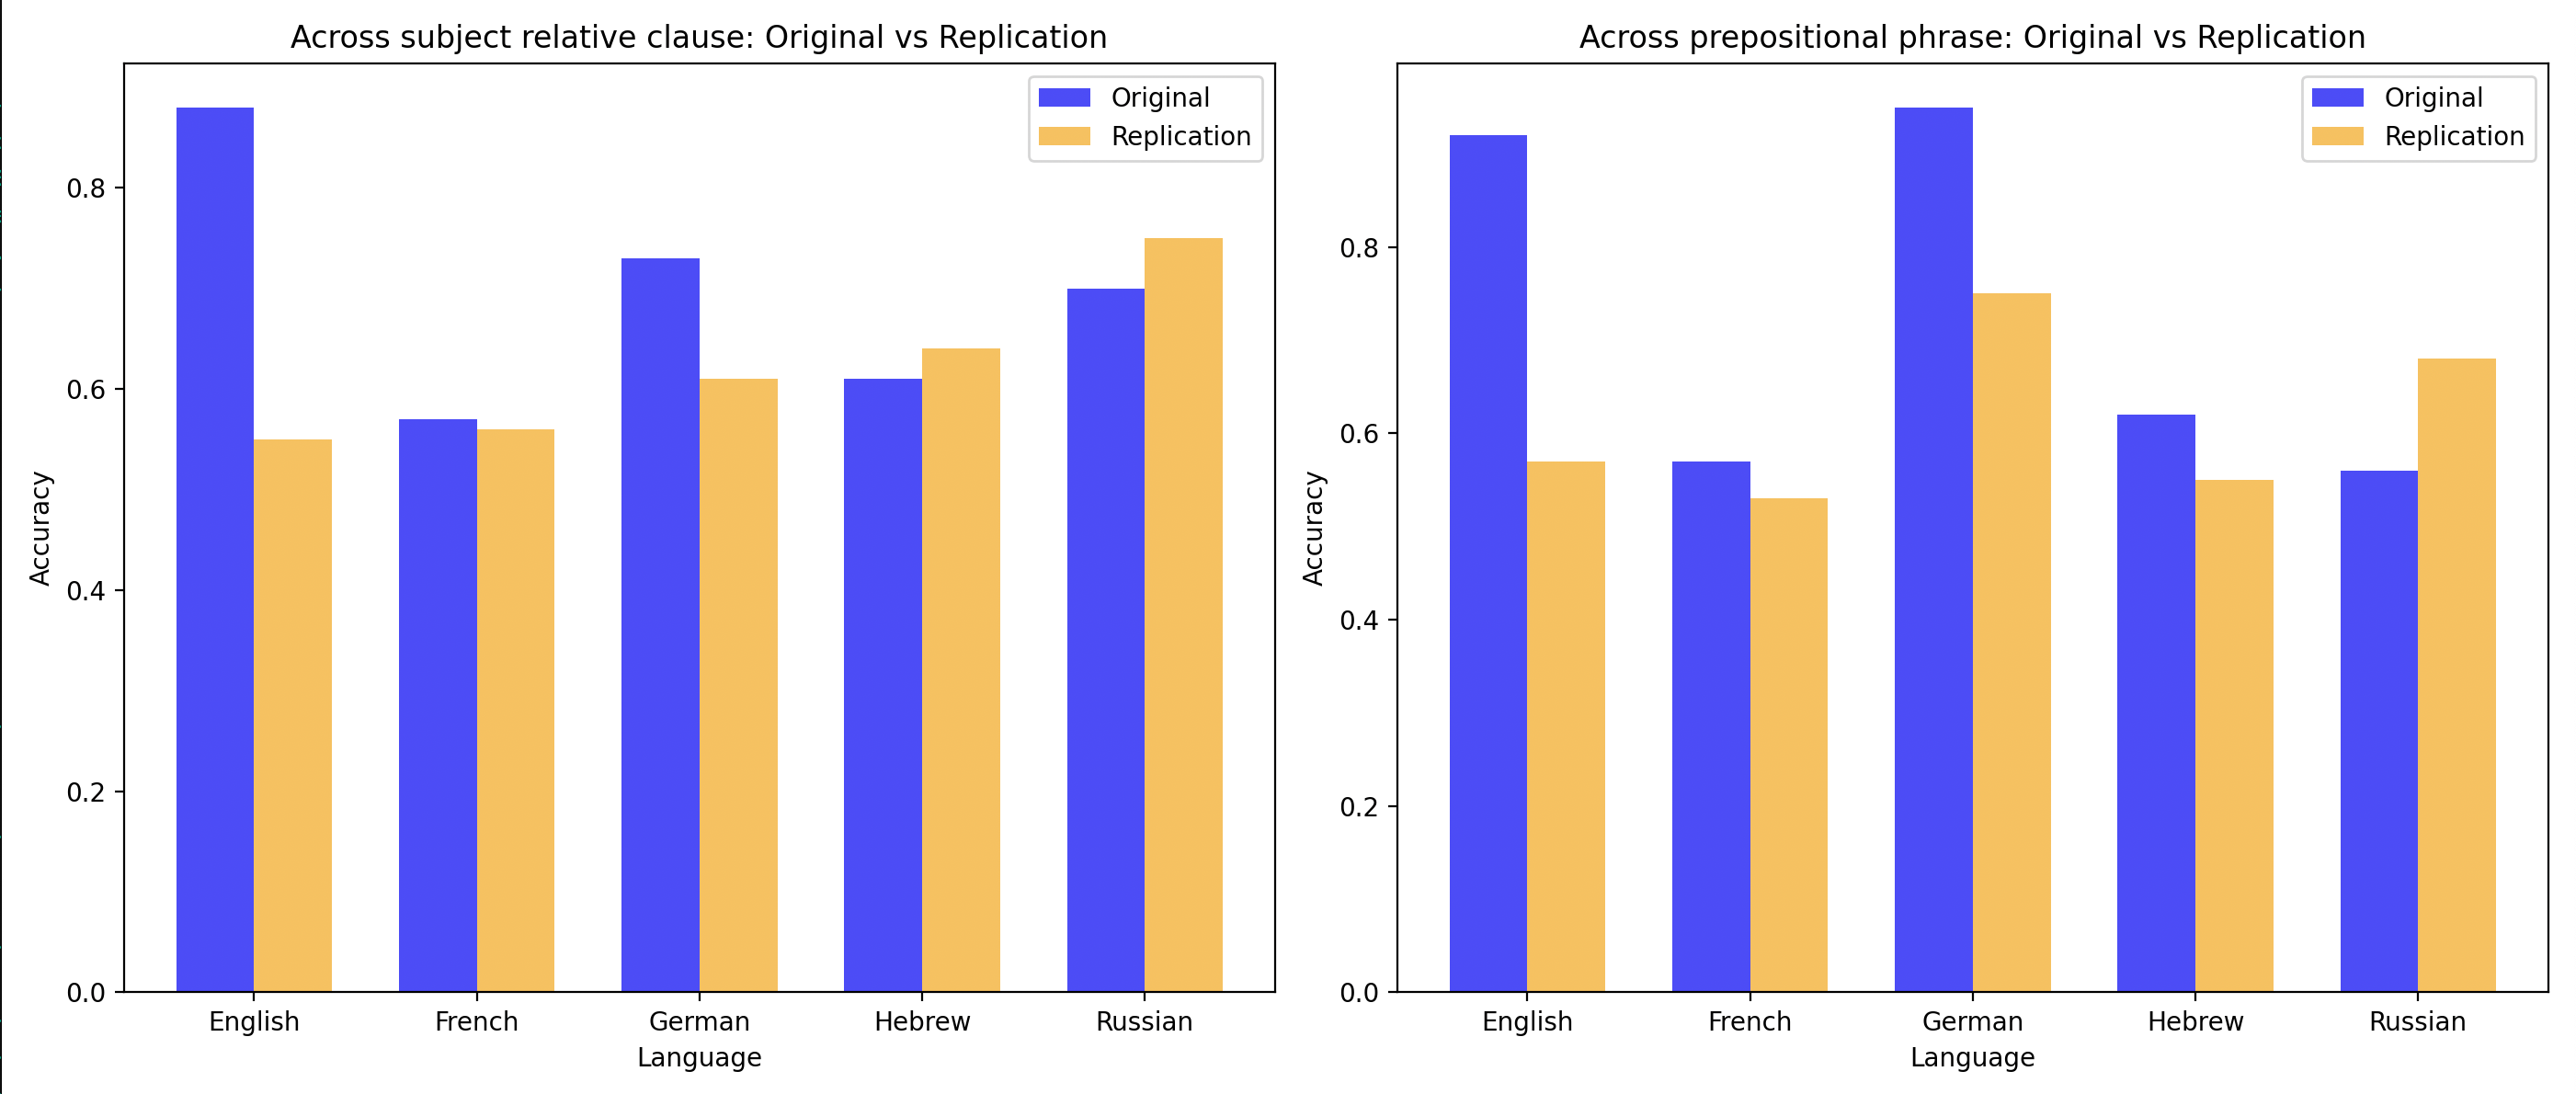
\includegraphics[width=0.45\textwidth]{sr_prep_compare.png}
    \caption{Accuracy Comparison Across Subject Relative Clauses and Prepositional Phrases: Original vs Replication Across Languages}
    \label{fig:sr_pp_comparison}
\end{figure}

When analyzing complex syntactic structures, performance varied significantly across different languages. In the case of \textit{across subject relative clauses}, Hebrew and Russian exhibited better performance (0.64 and 0.75, respectively) compared to English (0.55) and French (0.56). The differences suggest that the model struggles more with these constructions in languages that share less structural similarity with English, potentially affecting the model’s ability to generalize across languages.

A similar pattern was observed for \textit{across prepositional phrases}, where German achieved the highest accuracy (0.75), followed by Russian (0.68). This may be due to the syntactic characteristics of German and Russian, where prepositional phrases are structured differently compared to English. These results further emphasize the challenges faced by multilingual models when dealing with language-specific grammatical rules, especially when those rules diverge significantly from the English-based training data used for BERT.


\paragraph{Mono vs Multi BERT Performance}
Both monolingual and multilingual BERT showed strong performance in simpler structures such as \textit{VP coordination (long)}, achieving accuracies of 0.98 and 0.87, respectively \autoref{tab:Table3}. However, as the syntactic complexity increased, accuracy noticeably declined for both models. For example, in \textit{across-subject relative clauses}, monolingual BERT outperformed multilingual BERT with an accuracy of 0.76 compared to 0.62 \autoref{tab:Table3}. This drop indicates that more complex dependencies between sentence elements, such as those found in relative clauses, are more challenging for both models, but especially for multilingual BERT.



Similarly, in \textit{within-object relative clauses}, monolingual BERT maintained a higher accuracy of 0.83, while multilingual BERT achieved only 0.60 \autoref{tab:Table3}. This consistent performance gap between the two models across different sentence structures suggests that monolingual BERT is better at capturing and generalizing syntactic rules within a single language, likely because it is trained on more language-specific data. In contrast, multilingual BERT, while versatile across multiple languages, may struggle with deep syntactic nuances due to the trade-offs made during multilingual training.


Interestingly, unlike the original study, where hyphens were used to indicate out-of-vocabulary cases for certain constructions (e.g., \textit{Within object relative clause} in Hebrew and \textit{VP coordination} (long)" in Russian, our replication successfully computed results for these constructions. This suggests that modifications in our dataset preparation or model training—such as enhanced preprocessing for better word coverage or fine-tuning—may have improved the models' ability to handle these previously problematic cases. By generating results for these constructions, our replication offers a more comprehensive evaluation of syntactic structures across multiple languages.

These results highlight that although multilingual models are useful for handling multiple languages, they still face challenges in mastering the intricacies of complex syntactic structures. This is likely because the training data for multilingual BERT must generalize across languages, which may dilute its ability to focus on language-specific syntactic rules. Monolingual BERT, on the other hand, benefits from language-specific data, allowing it to perform more accurately in these complex syntactic scenarios.

\begin{figure}[htbp]
    \centering
    \includegraphics[width=0.45\textwidth]{monoVSmulti.png}
    \caption{Comparison of Mono vs Multi BERT Performance - Replication vs Original}
    \label{fig:mono-vs-multi}
\end{figure}

Overall the average results of our models, monolingual BERT and mBERT,were lower but still close to the orginial study's results, as seen in \autoref{fig:mono-vs-multi}.

\section{Discussion}
The main motivation behind our paper was to replicate a cross-linguistic syntactic evaluation, using the same dataset, investigating how word prediction models perform across multiple languages. We hypothesized that our more expansive dataset with matching syntax in different languages would provide more data for these models to learn from. 

In our results as can be seen in \autoref{tab:Table3}, we observed better performance for monolingual BERT and multilingual BERT on simpler structures like \textit{Simple} (mono: 0.79, multi: 0.78), \textit{VP (short)} (mono: 0.89, multi: 0.81), and \textit{VP (long)} (mono: 0.98, multi: 0.87), similar to the original study \autoref{fig:mono-vs-multi}. For more complex structures, though, both models had lower accuracy, aligning with the results from the original paper and supporting their conclusions that BERT models can learn from multiple languages for simpler sentence structures. However, we did not have as strong of evidence to conclude that some languages perform far better than others.

One notable difference in our replication is that we were able to compute results for constructions where the original study used hyphens to indicate out-of-vocabulary cases, such as \textit{Within object relative clause} in Hebrew and \textit{VP coordination (long)} in Russian. This improvement is likely due to modifications we made during dataset preprocessing to fit the \textit{NLPScholar} format. The changes we made ensured better compatibility and may have enhanced word coverage, allowing the models to handle previously out-of-vocabulary cases. Additionally, \textit{NLPScholar}’s evaluation processes may have contributed to these improvements by facilitating more robust comparisons across sentence structures.

Both the original study and our replication focus on only five languages and on a specific set of subject-verb sentence structures. While the limited number of languages and sentence structures made it easier to compare performance across languages, it also restricted the variety of sentences tested. In other words, there are other sentence structures that may have yielded useful insights that we could not test. Also, using \textit{NLPScholar} in our replication may have impacted how the models processed and evaluated certain sentences, explaining some of the discrepancies we observed compared to the original study.

Our replication results support the original study's conclusions about monolingual and multilingual BERT. The multilingual models can apply syntax rules across languages, but they struggle with more complex sentence structure, and monolingual BERT consistently outperformed the multilingual BERT. Following the recommendations from the original paper, we agree that future work could explore architectural changes or fine-tuning on non-Latin script languages to enhance performance further.

\section*{Acknowledgements}

\begin{figure}[htbp]
    \centering
    \includegraphics[width=0.45\textwidth]{cat.png}
    \caption{\url{https://xkcd.com/262/}}
    \label{fig:cat}
\end{figure}


\bibliography{anthology,custom}
\bibliographystyle{acl_natbib}

\end{document}
